\documentclass{article}
% basics
\usepackage{amsfonts}
\usepackage{enumitem}
\usepackage{float}
\usepackage{graphicx}
\usepackage{hyperref} 
\usepackage[labelfont=bf]{caption}

\newtheorem{theorem}{Theorem}
\newtheorem{lemma}[theorem]{Lemma}
\newtheorem{corollary}{Corollary}[theorem]

% unique math expressions:  
\usepackage{amsmath}
\DeclareMathOperator*{\andloop}{\wedge}
\DeclareMathOperator*{\pr}{Pr}
\DeclareMathOperator*{\approach}{\longrightarrow}
\DeclareMathOperator*{\eq}{=}

% grey paper
\usepackage{xcolor}
% \pagecolor[rgb]{0.11,0.11,0.11}
% \color{white}

% embedded code sections
\usepackage{listings}
\definecolor{codegreen}{rgb}{0,0.6,0}
\definecolor{codegray}{rgb}{0.5,0.5,0.5}
\definecolor{codepurple}{rgb}{0.58,0,0.82}
\lstdefinestyle{mystyle}{
    commentstyle=\color{codegreen},
    keywordstyle=\color{magenta},
    numberstyle=\tiny\color{codegray},
    stringstyle=\color{codepurple},
    basicstyle=\ttfamily\footnotesize,
    breakatwhitespace=false,         
    breaklines=true,                 
    captionpos=b,                    
    keepspaces=true,                 
    numbers=left,                    
    numbersep=5pt,                  
    showspaces=false,                
    showstringspaces=false,
    showtabs=false,                  
    tabsize=2
}

\lstset{style=mystyle}

\begin{document}
\author{Yosef Goren \& Yonatan Kahalani}
\title{Database Systems - Homework 4}
\maketitle


\section{}
\subsection{}
\begin{lstlisting}
for all tuples s in S:
    for all tuples  a in A:
        if a.artistID == A.ID and A.genre == 'Jazz' and
                s.releaseDate>=TO_DATE('2023/00/00','YYYY/MM/DD'):
            output(a.ID, s.ID)
\end{lstlisting}
Let $B_A$ be the number of blocks in $A$,
$B_S$ the number of blocks in $S$ and $n_S$
the number of tuples in $S$.\\
As seen in the lectures the IO
cost for this is $O(B_A+n_S\cdot B_S)=O(10^4+10^7)$

\subsection{}
\begin{enumerate}[label=\roman*.]
    \item IO cost $O(1)$. By going through the tree and
    and finding the lexicographically largest element with
    the constraint that \texttt{artistID=236363}, then getting
    the block which contains it - and extracting that element from that block.
    \item
    \label{}
    Let $n_S$ be the number of rows that refer to this artirst,
    from the year $2023$ onwards. Thus the IO complexity is $O(n_S)$.\\
    After going to the index and finding the largest leaf with $artistID=236363$,
    we can generate the set of outputs (while outputing the \texttt{s.id} for each tuple) in decending order
    by iterating over
    the leaves which have a year after $2023$.\\
    Note that the specific ordering is not required by the implementation is more efficient this way.
\end{enumerate}

\subsection{}
Iterate over each element from the set of artits,
if the artist's genre is Jazz - output all of his songs which are from after $2023$ -
by searching through the tree in lexicographic order - in the same way as in \ref{} (Denote this alg with \texttt{alg12}),
and finally we project the tuples on \texttt{A.ID} and \texttt{S.ID}.
\begin{lstlisting}
for all tuples a in A:
    if a.genre == 'Jazz':
        //run alg from 1.2 ii running on a
        T := alg12(a)
        for t in T:
            output(a.id, t.id)
\end{lstlisting}


\section{}
\subsection{}

\begin{enumerate}[label=\roman*.]
    \item 
    First we show the scheduling is not \emph{view serializable}
    and thus it is not \emph{conflict serializable} - thanks to the theorem
    seen in lectures which states that conflict serializability implies view serializability.\\

    First we note that in any serial scheduling which is equivalent to the given scheduling,
    $T_3$ has be come after $T_2$ since $T_3$ and $T_2$ refer to the same variable $y$.\\
    Thus the scheduling options remaining are:
    \begin{enumerate}
        \item $T_1\rightarrow T_2\rightarrow T_3$.\\
        This scheduling is not equivalent since in the original
        schedule - $T_1$ reads $y$ written by $T_2$ and in this one it reads the initial value of $y$.
        \item $T_2\rightarrow T_3\rightarrow T_1$\\
        Not equivalent since in the original the final value of $x$ is written by $T_2$
        while in this schedule it is written by $T_1$.
        \item $T_2\rightarrow T_1\rightarrow T_3$\\
        Not equivalent due to exact the same reason as $T_2\rightarrow T_3\rightarrow T_1$.
    \end{enumerate}
    \item  Denote the following serialization:
    $$
    S'=R_2(z), R_2(y), W_2(x), W_3(z), W_4(z), R_4(y), R_1(z)
    $$
    The operations are equivalent: $S=_CS'$, since each pair of operations
    in conflict in $S$ appear in the same relative order in $S'$.\\
    For example the
    conflicting operations $R_2(z), W_3(z)$, are in the ordering\\
    $R_2(z)\rightarrow ...\rightarrow W_3(z)$
    both in the original and new schedule.\\
    
    Thus $S$ is \emph{conflict serializable} by def.\\
    Thus from the theorem seen in lecture - $S$ is also \emph{view serializable}.

    \item Denote the provided schedule as $S$.\\
    Note that $T_2$ is has to appear last in any serial scheduling
    which is equivalent to the one provided, since all transactions write to $y$,
    while $W_2(y)$ happends after both $W_1(y)$ (meaning $T_2$ must be after $T_1$) and
    $W_2(y)$ is after $W_3(y)$ (meaning $T_2$ must be after $T_3$).\\
    Thus we are left with two options:
    \begin{enumerate}
        \item $T_1\rightarrow T_3\rightarrow T_2$
        \item $T_3\rightarrow T_1\rightarrow T_2$
    \end{enumerate}
    $b$ is not \emph{view equivalent} to $S$ since
    $S$, $T_1$ reads $y$'s initial value, while in $b$ -
    $T_1$ reads the value written to $y$ in $T_3$.\\
    $a$ is \emph{view equivalent} to $S$ by def. and thus
    $S$ is \emph{view serializable}.\\
    So far we have found that $a$ is the only possbile equivalent serialization of
    $S$. Since in $S$: $W_3(y)\rightarrow\cdots\rightarrow W_1(y)$,
    and in $a$: $W_1(y)\rightarrow\cdots\rightarrow W_3(y)$,
    thus $a$ is not \emph{conflict equivalent} to $S$.\\
    This means there is no \emph{conflict equivalent} serialization for $S$.\\
    Hence $S$ is not \emph{conflict serializable}.
\end{enumerate}

\subsection{}
\begin{enumerate}[label=\roman*.]
    \item $R_{L_1}(x), R_{1}(x), R_{L_2}(y), R_{2}(y), R_{1}(x), R_{U_1}(x), R_{L_2}(x), R_{2}(x), R_{2}(y), R_{U_2}(x), R_{U_2}(y)$
    \item $W_2(x), W_1(x), W_2(x), R_2(y)$
\end{enumerate}

\section{}
For the purpose of providing an example for each
solution we have provided in this question we have
created an example database and added a few kittens to it, and ran the
solution queries on each of them.\\
The following code creates the content of our databse:
\begin{lstlisting}
CREATE (b1:Breed {name: 'Siamese', origin: 'Thailand', lifespan: '12-15 years'})
CREATE (b2:Breed {name: 'Bengal', origin: 'United States', lifespan: '12-16 years'})
CREATE (b2)-[:DESCENDANT_OF]->(b1)

CREATE (o1:Owner {name: 'John Smith', address: '123 Main St'})
CREATE (o2:Owner {name: 'Emily Johnson', address: '456 Elm St'})

CREATE (c1:Cat {name: 'Max', age: 3, gender: 'Male'})
CREATE (c2:Cat {name: 'Luna', age: 2, gender: 'Female'})
CREATE (c3:Cat {name: 'Oliver', age: 4, gender: 'Male'})
CREATE (c4:Cat {name: 'Chloe', age: 1, gender: 'Female'})
CREATE (c5:Cat {name: 'Hatol', age:7, gender: 'Male'})

CREATE (c1)-[:BELONGS_TO {relationship_length: 2}]->(o1)
CREATE (c2)-[:BELONGS_TO {relationship_length: 1}]->(o1)
CREATE (c3)-[:BELONGS_TO {relationship_length: 1}]->(o2)
CREATE (c4)-[:BELONGS_TO {relationship_length: 1}]->(o2)
CREATE (c5)-[:BELONGS_TO {relationship_length: 3}]->(o1)

CREATE (c1)-[:OF_BREED]->(b1)
CREATE (c2)-[:OF_BREED]->(b1)
CREATE (c3)-[:OF_BREED]->(b2)
CREATE (c4)-[:OF_BREED]->(b2)
CREATE (c5)-[:OF_BREED]->(b2)
\end{lstlisting}
Here is how the graph looks after adding the kittens:\\
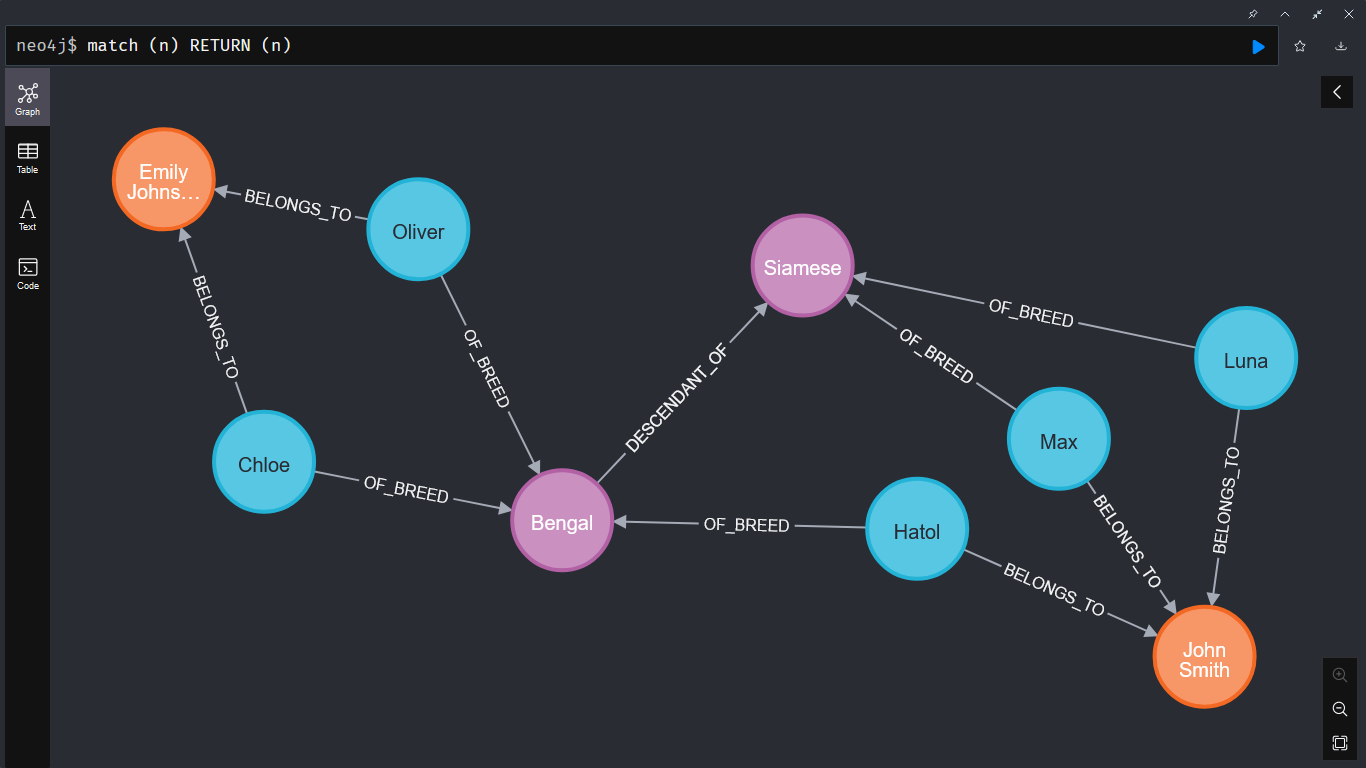
\includegraphics[width=\textwidth]{kittens1.png}

\subsection{}
The query can be solved by:
\begin{lstlisting}
MATCH (b:Breed)
OPTIONAL MATCH (b)<-[:OF_BREED]-(c:Cat)
RETURN b.name, count(c)
\end{lstlisting}

Running this on our example yields:\\
\begin{center}
\begin{tabular}{|c|c|}
    \hline
    \textbf{b.name} & \textbf{count(c)} \\
    \hline
    "Siamese" & 2 \\
    \hline
    "Bengal" & 3 \\
    \hline
\end{tabular}
\end{center}
  

\subsection{}
This question is solved by the query:
\begin{lstlisting}
MATCH (o:Owner)<-[:BELONGS_TO]-(c:Cat)-[:OF_BREED]->(b:Breed)
WITH o, collect(DISTINCT b) AS breeds
WHERE size(breeds) = 1
RETURN o.name
\end{lstlisting}

Running this on our example yields:\\
\begin{center}
\begin{tabular}{|c|c|}
    \hline
    \textbf{b.name} & \textbf{count(DISTINCT c)} \\
    \hline
    "Siamese" & 5 \\
    \hline
    "Bengal" & 3 \\
    \hline
\end{tabular}
\end{center}
  

\subsection{}
This question is solved by the query:
\begin{lstlisting}
MATCH (b:Breed)
OPTIONAL MATCH (b)<-[:DESCENDANT_OF*0..]-(:Breed)-[:OF_BREED]-(c)
RETURN b.name, count(DISTINCT c)    
\end{lstlisting}

Running this on our example yields:\\
\begin{center}
\begin{tabular}{|c|}
    \hline
    \textbf{o.name} \\
    \hline
    "Emily Johnson" \\
    \hline
\end{tabular}
\end{center}


\subsection{}
This question is solved by the query:
\begin{lstlisting}
MATCH (b:Breed)
OPTIONAL MATCH (b)<-[:OF_BREED]-(c:Cat)
RETURN b.name, count(c)
\end{lstlisting}

Running this on our example yields:\\
\begin{center}
\begin{tabular}{|c|}
    \hline
    \textbf{o.name} \\
    \hline
    "John Smith" \\
    \hline
\end{tabular}
\end{center}

\end{document}